\vspace*{-0.5em}\section{Related work}\vspace*{-0.5em}
\label{sec:related}

\begin{figure*}  % This is supposed to be in methods, but putting it here to force it to be on page 3
  \centering
  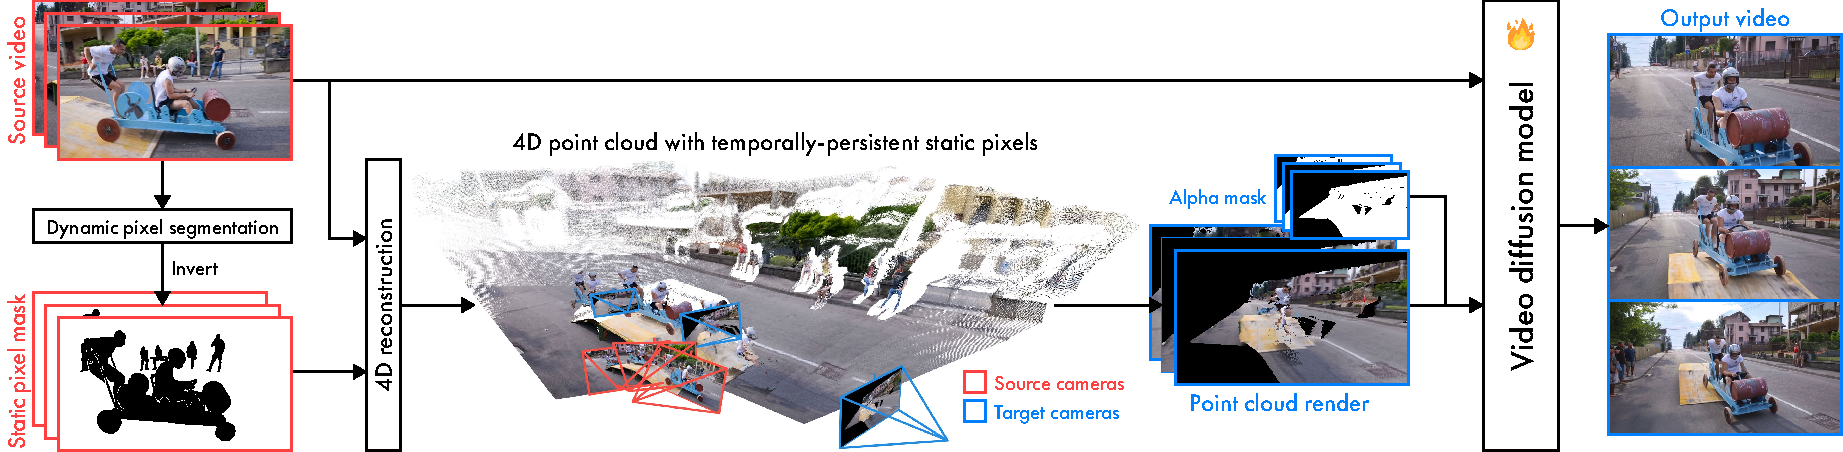
\includegraphics[width=\textwidth]{figures/mid_res/pipeline.pdf}
  \caption{\Paragraphnoskip{Overview of \methodname} Given an input source video, we build a 4D point cloud where static pixels are temporally persistent via segmentation and 4D reconstruction. We then render the point cloud in the target cameras which users define. Lastly, the source video and point cloud render \& alpha mask are jointly processed by the finetuned video diffusion model to generate a video of the same dynamic scene in the target cameras. We provide model architecture details in  Supplementary \ref{supp:architecture}.}
  \label{fig:pipeline}
\end{figure*}

\begin{figure}
  \centering
  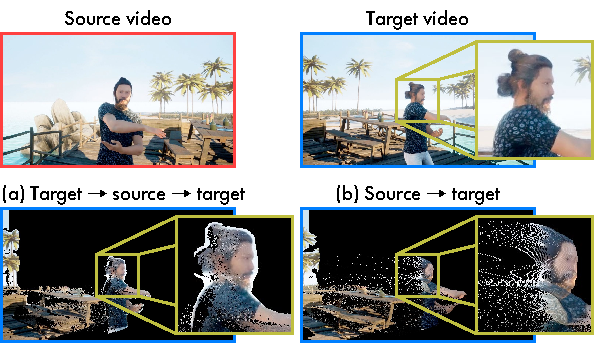
\includegraphics[width=\columnwidth]{figures/mid_res/multiview.pdf}
  \caption{\Paragraphnoskip{Multiview 4D reconstruction artifacts} (a) Double reprojection \cite{yu2025trajcraft} first renders the target video point cloud in the source camera, then rerendering it in the target camera to create occluded regions for paired training, thus viewing the target video depth map from its frontal, artifact-free view. (b) In contrast, rendering the source video point cloud from the target camera with dynamic multiview data exposes non-frontal-view artifacts that better match real-world inference. The above source-target video pair is from MultiCamVideo \cite{bai2025recammaster} with 4D reconstruction by STream3R \cite{lan2025stream3r}.}
  \label{fig:multiview}
\end{figure}

\Paragraph{Video reshooting with \emph{explicit priors}}
For video reshooting, and more broadly novel view synthesis of static scenes, 3D/4D point clouds provide an explicit and rich spatial prior. To this end, video reshooting methods with \emph{explicit priors} \cite{ren2025gen3c, yu2025trajcraft, hu2025ex4d, jeong2025reangle, you2025nvssolver, qian2025wristworld} use video depth estimators \cite{chen2025videodepthanything, hu2025depthcraft, xu2025geocraft} to render per-frame camera-space point clouds as conditioning signals for video diffusion models. Depth estimation priors have also been widely used for static scene novel view synthesis (NVS) \cite{kant2023invs, muller2024multidiff} and video motion control \cite{xiao2025trajattn, ren2025gen3c}. However, many of these methods often train on precise depth maps which inhibits generalization to imperfect real-world depth estimation, and their per-frame point cloud conditioning can struggle to preserve seen content and maintain accurate camera control with challenging camera trajectories.

\Paragraph{Video reshooting with \emph{implicit priors}}
Alternatively, video shooting methods can also use \emph{implicit priors} for camera control such as camera embeddings \cite{bai2025recammaster, vanhoorick2024gcd} or video references \cite{luo2025camclonemaster} by finetuning video diffusion models on time-synchronized synthetic multiview data. Image- and camera-conditioned diffusion models have also been used for static scene NVS~\cite{zhou2025seva, kant2024spad, liu2023zero123, shi2023mvdream,voleti2024sv3d} and camera-controlled video generation \cite{he2025cameractrlii,bahmani2024vd3d,xie2024sv4d}. However, due to the inherent depth scale ambiguity of monocular videos, camera control from implicit-prior methods is often imprecise and unable to be explicitly `previewed' unlike point clouds.

\Paragraph{4D reconstruction}
To provide explicit geometric priors for video reshooting, we lift the input video into a world-space point cloud with 4D reconstruction. Traditional structure from motion~\cite{schonberger2016colmap,wang2024vggsfm, pan2024glomap} rely on multiview geometry constraints but are not robust to dynamic scenes. With the strong performance of learning-based video depth estimation models~\cite{chen2025videodepthanything, hu2025depthcraft, xu2025geocraft, chou2025flashdepth,wang2025moge, piccinelli2025unidepthv2}, recent works \cite{li2025megasam, yao2025uni4d, huang2025vipe} combine these depth priors and camera optimization with SLAM~\cite{teed2021droid} to obtain robust and coherent dynamic scene reconstruction. Followed by recent success in end-to-end 3D reconstruction methods~\cite{wang2024dust3r, wang2025vggt, keetha2025mapanything}, end-to-end 4D reconstruction models~\cite{wang2025pi3, lan2025stream3r, sun2024monst3r, zhuo2025stream4dvgt, jiang2025geo4d} have also emerged as more efficient alternatives. Some recent methods also predict 4D Gaussians from monocular videos~\cite{lei2025mosca, wang2025shapeofmotion, wang2025gflow}, enabling novel view synthesis at small viewpoint deviations from the input videos.
